%%%%%%%%%%%%%%%%%%%%%%%%%%%%%%%%%%%%%%%%%
% baposter Landscape Poster
% LaTeX Template
% Version 1.0 (11/06/13)
%
% baposter Class Created by:
% Brian Amberg (baposter@brian-amberg.de)
%
% This template has been downloaded from:
% http://www.LaTeXTemplates.com
%
% License:
% CC BY-NC-SA 3.0 (http://creativecommons.org/licenses/by-nc-sa/3.0/)
%
%%%%%%%%%%%%%%%%%%%%%%%%%%%%%%%%%%%%%%%%%
%----------------------------------------------------------------------------------------
%	PACKAGES AND OTHER DOCUMENT CONFIGURATIONS
%----------------------------------------------------------------------------------------

\documentclass[landscape,paperwidth=42in,paperheight=36in,fontscale=0.32]{baposter} % Adjust the font scale/size here

\usepackage{graphicx} % Required for including images
\graphicspath{{figures/}} % Directory in which figures are stored

\usepackage{amsmath} % For typesetting math
\usepackage{amssymb} % Adds new symbols to be used in math mode

\usepackage{booktabs} % Top and bottom rules for tables
\usepackage{enumitem} % Used to reduce itemize/enumerate spacing
\usepackage{palatino} % Use the Palatino font
\usepackage[font=small,labelfont=bf]{caption} % Required for specifying captions to tables and figures

\usepackage{multicol} % Required for multiple columns
\setlength{\columnsep}{1.5em} % Slightly increase the space between columns
\setlength{\columnseprule}{0mm} % No horizontal rule between columns

\usepackage{tikz} % Required for flow chart
\usetikzlibrary{shapes,arrows} % Tikz libraries required for the flow chart in the template

\newcommand{\compresslist}{ % Define a command to reduce spacing within itemize/enumerate environments, this is used right after \begin{itemize} or \begin{enumerate}
\setlength{\itemsep}{1pt}
\setlength{\parskip}{0pt}
\setlength{\parsep}{0pt}
}

\definecolor{lightblue}{rgb}{0.145,0.6666,1} % Defines the color used for content box headers

\begin{document}

\begin{poster}
{
headerborder=closed, % Adds a border around the header of content boxes
colspacing=1em, % Column spacing
bgColorOne=white, % Background color for the gradient on the left side of the poster
bgColorTwo=white, % Background color for the gradient on the right side of the poster
borderColor=lightblue, % Border color
headerColorOne=black, % Background color for the header in the content boxes (left side)
headerColorTwo=lightblue, % Background color for the header in the content boxes (right side)
headerFontColor=white, % Text color for the header text in the content boxes
boxColorOne=white, % Background color of the content boxes
textborder=roundedleft, % Format of the border around content boxes, can be: none, bars, coils, triangles, rectangle, rounded, roundedsmall, roundedright or faded
eyecatcher=true, % Set to false for ignoring the left logo in the title and move the title left
headerheight=0.1\textheight, % Height of the header
headershape=roundedright, % Specify the rounded corner in the content box headers, can be: rectangle, small-rounded, roundedright, roundedleft or rounded
headerfont=\Large\bf\textsc, % Large, bold and sans serif font in the headers of content boxes
textfont={\setlength{\parindent}{1.5em}}, % Uncomment for paragraph indentation
linewidth=2pt % Width of the border lines around content boxes
}
%----------------------------------------------------------------------------------------
%	TITLE SECTION 
%----------------------------------------------------------------------------------------
%
{
\includegraphics[height=5em]{seas_logo}} % First university/lab logo on the left
{\bf\textsc{PM2.5 Exposure of Food Truck Workers}\vspace{0.5em}} % Poster title
{\textsc{\ Briana Franco, Justin Ebem, and Benjamin Schwartz \ \hspace{12pt} Columbia University \hspace{12pt} Chemical Engineering}} % Author names and institution
{
\includegraphics[height=5em]{seas_logo}} % Second university/lab logo on the right

%----------------------------------------------------------------------------------------
%	OBJECTIVES
%----------------------------------------------------------------------------------------

\headerbox{Objectives}{name=objectives,column=1,row=0}{

This study is designed to quantify the risk of PM2.5 exposure for food truck workers in Manhattan. The study will focus on ten food trucks, and characterize their exposure through a series of monitors in and around the truck. Each monitor will help to generate a map of where the sources of PM2.5 exposure are coming from, and the severity of the exposure. 
 

\begin{enumerate}\compresslist
\item Measure PM2.5 on the person
\item PM2.5 levels from the energy source at the truck
\item Measure traffic and ambient air contributions 
\item Characterize cooking aerosols
\item Generate overall idea of exposure
\end{enumerate}

\vspace{0.3em} % When there are two boxes, some whitespace may need to be added if the one on the right has more content
}

%----------------------------------------------------------------------------------------
%	INTRODUCTION
%----------------------------------------------------------------------------------------

\headerbox{The Problem}{name=introduction,column=0,row=0,bottomaligned=objectives}{

Manhattan food truck workers are surrounded by well documented sources of PM2.5: traffic, indoor cooking, and energy generation. The blending of both indoor and outdoor sources of PM2.5 creates a unique level of exposure with potentially more exposure and adverse health effects.
{\begin{center}
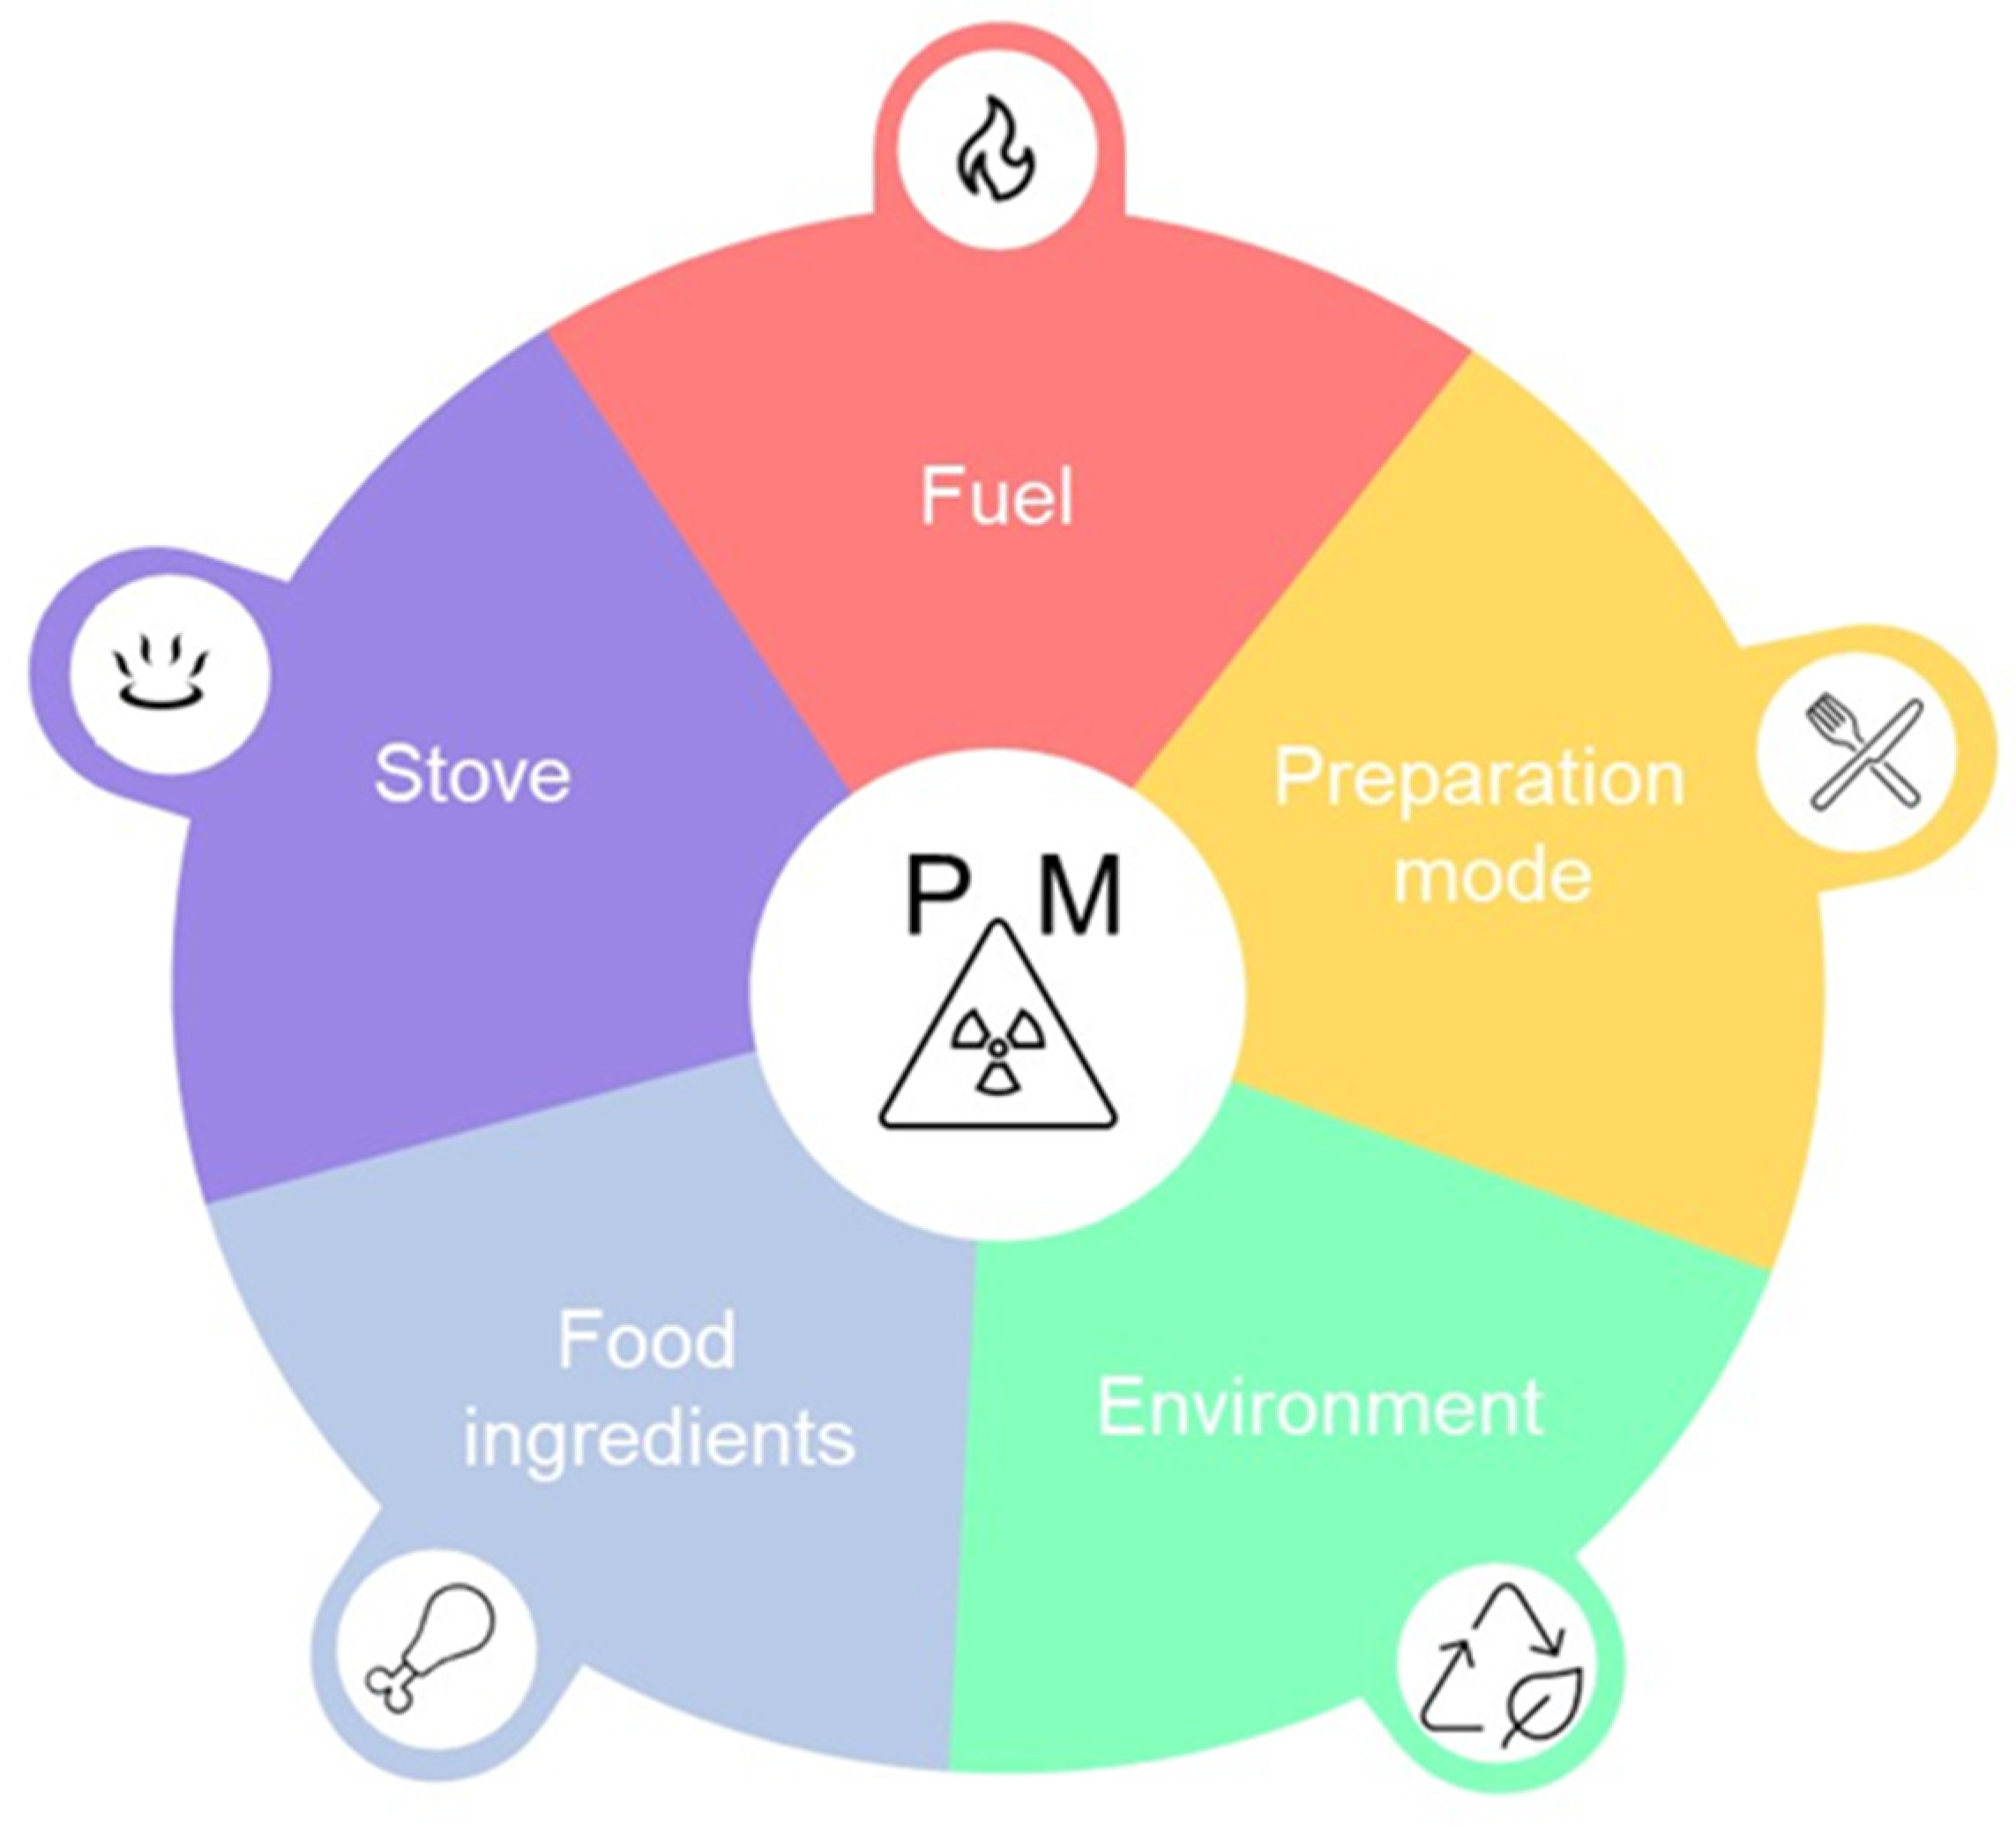
\includegraphics[width=0.50\linewidth]{exposure}
\captionof{figure}{Sources of PM (6)}
\end{center}}
}

%----------------------------------------------------------------------------------------
%	Literature Review and Motivation
%----------------------------------------------------------------------------------------

\headerbox{Literature Review and Motivation}{name=results,column=2,span=2,row=0}{

A literature review was conducted to identify PM2.5 sources to help inform the experimental setup. The first source that was evaluated was the cooking itself, and how cooking methods would impact the PM2.5 production. 

\begin{center}
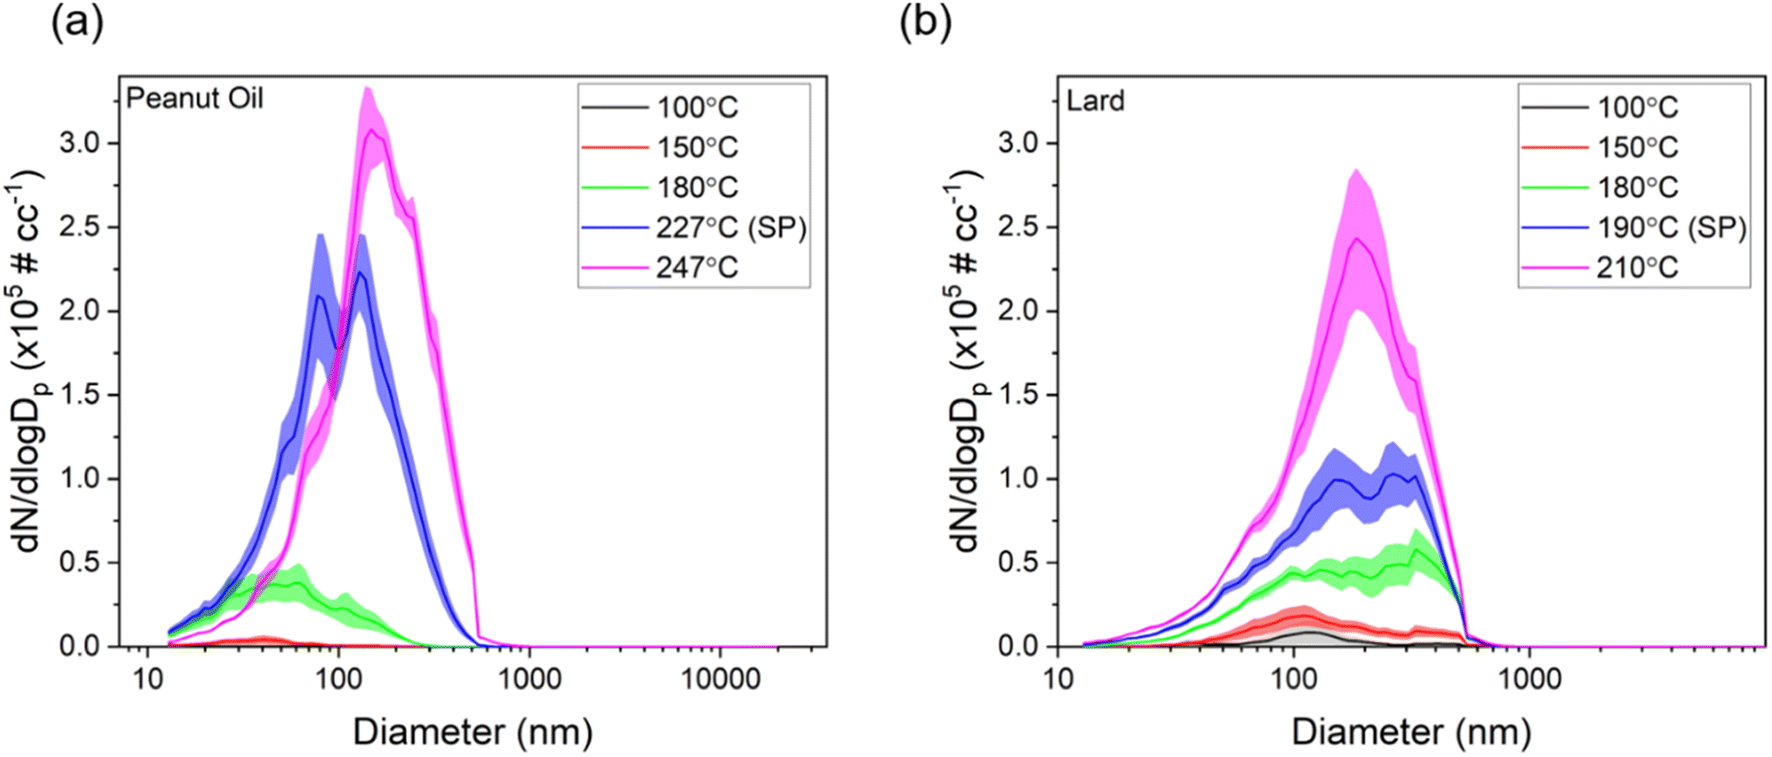
\includegraphics[width=0.7\linewidth]{cooking_temp}
\captionof{figure}{Differences in aerosol number size distribution as a function of cooking temperature for peanut oil and lard. (2)
}
\end{center}


The above chart displays the importance of cooking temperature on the amount of particulate produced. The disparity in PM2.5 production for different cooking temperatures motivates an investigation into how these various methods are impacting the cooks. 

\begin{center}
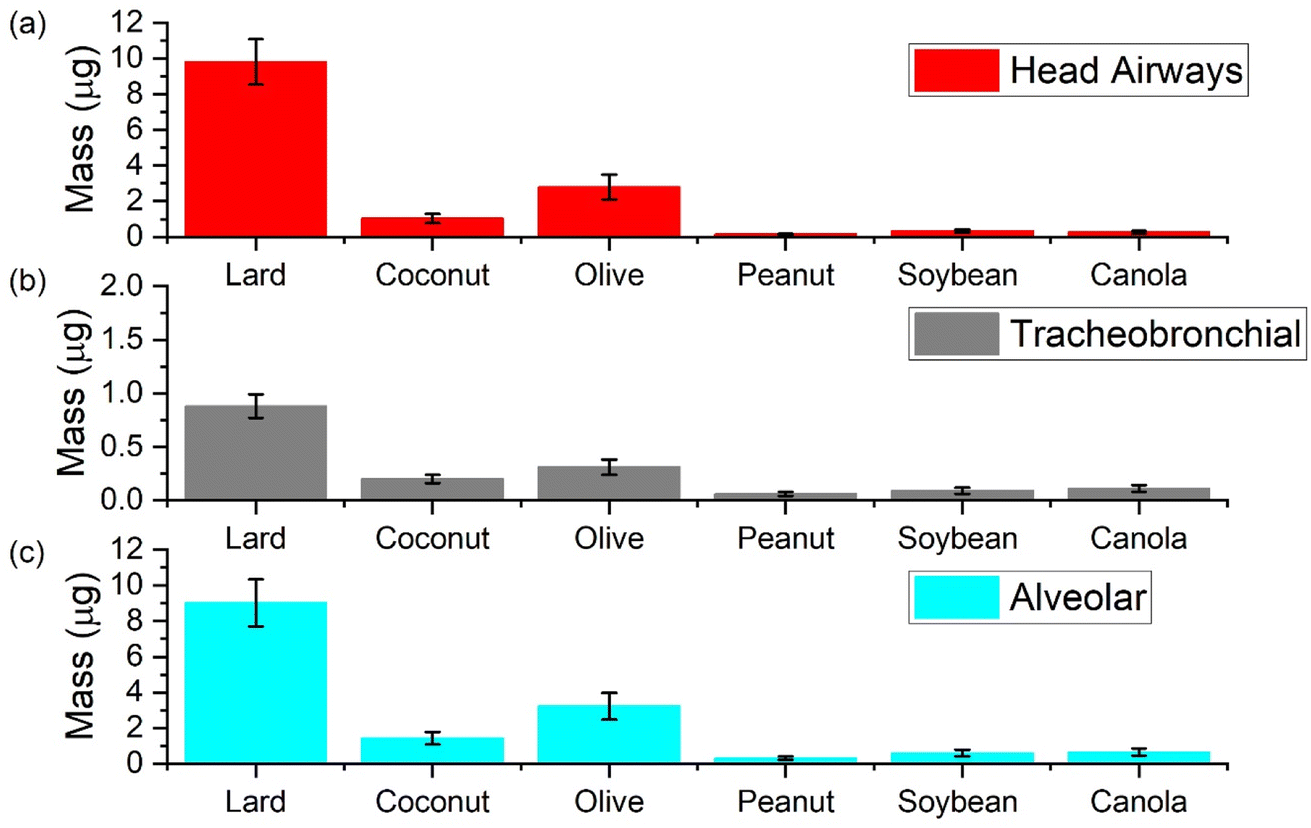
\includegraphics[width=0.44\linewidth]{cook}
\hfill
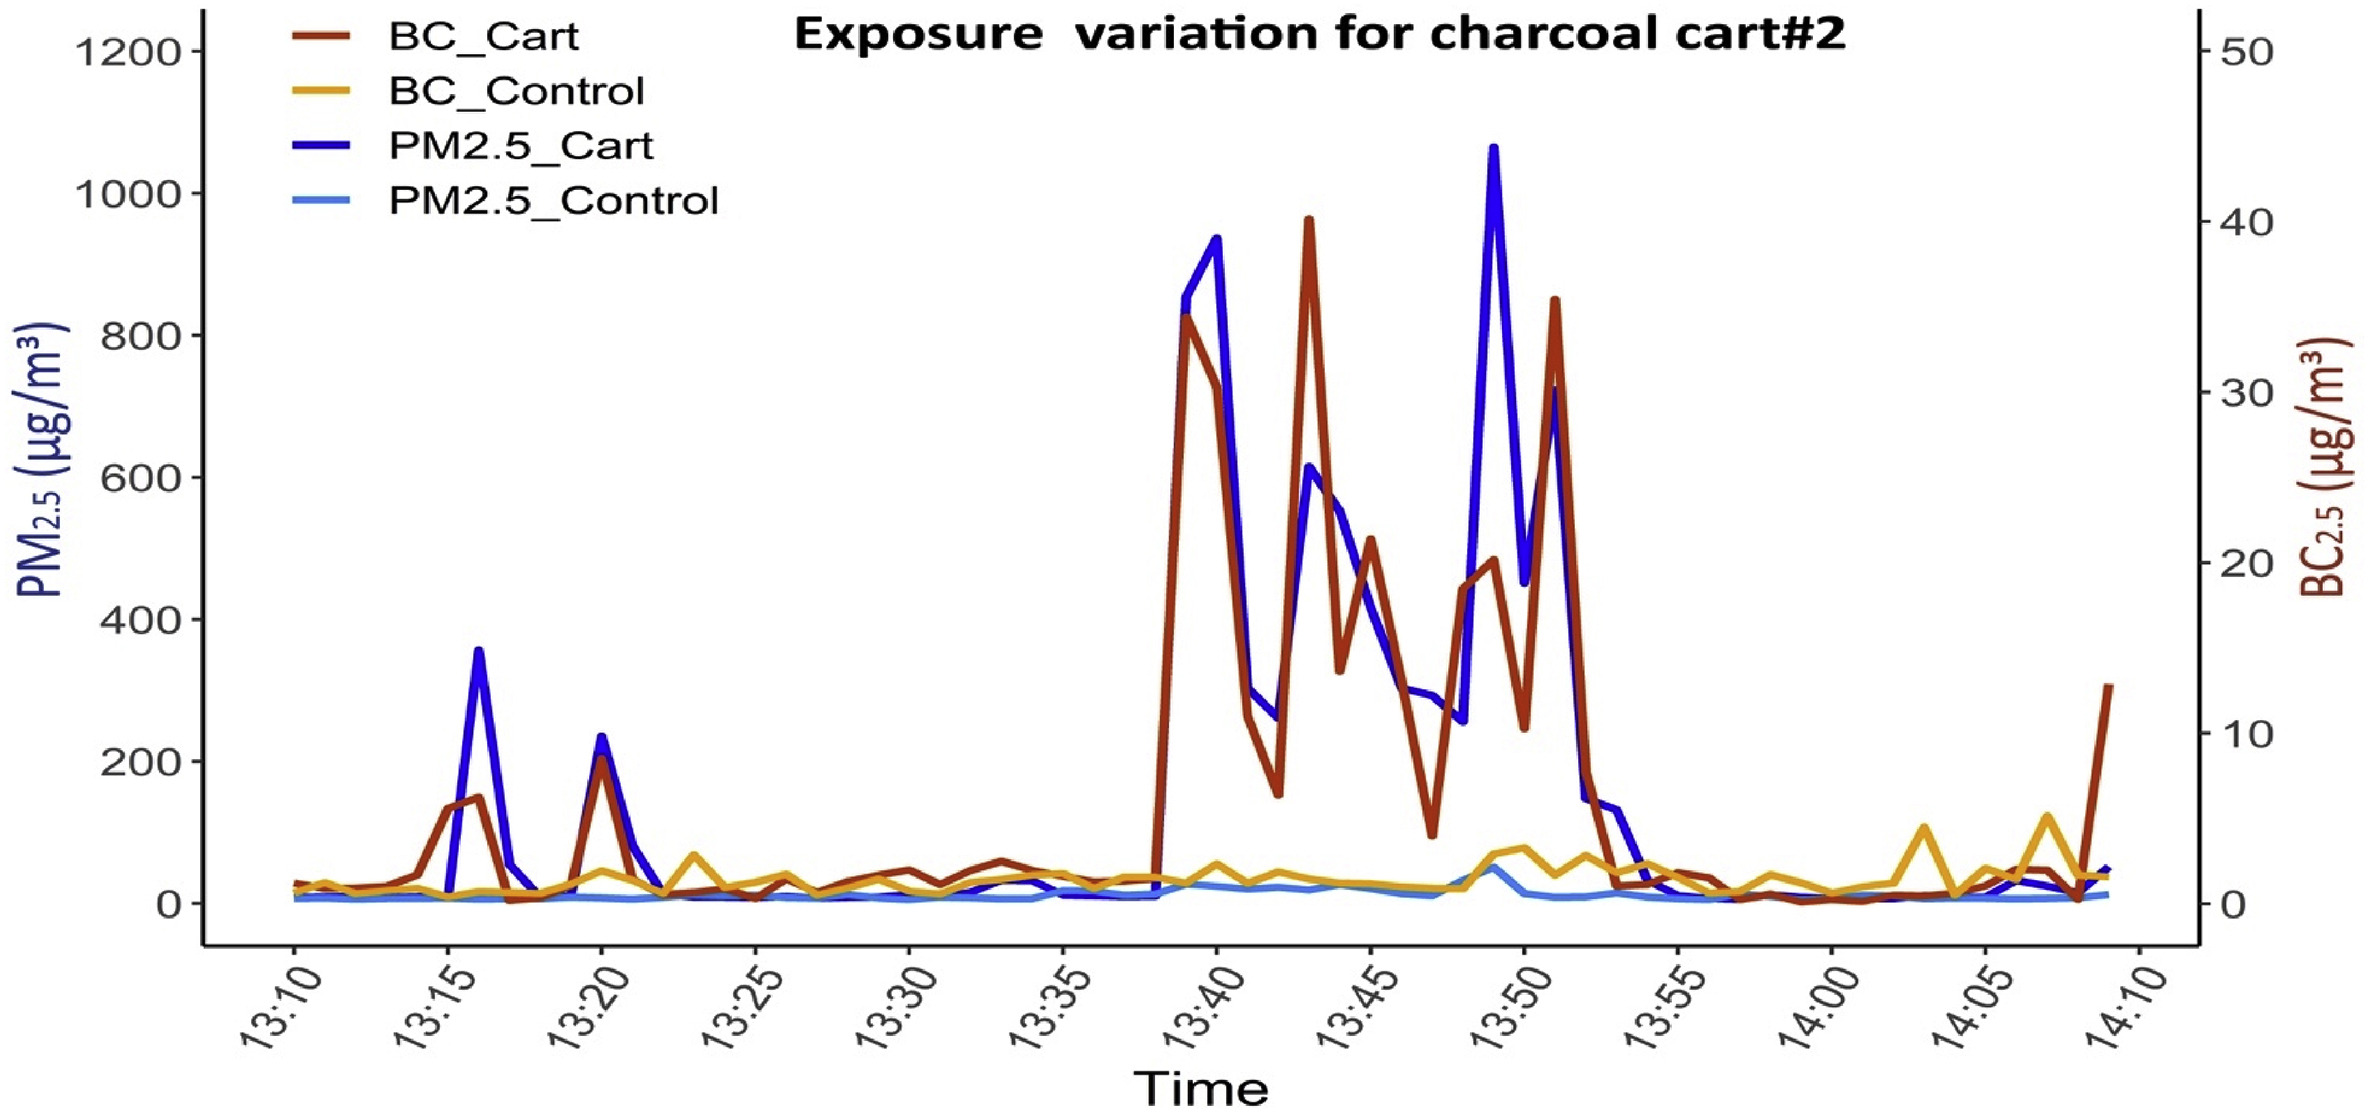
\includegraphics[width=0.5\linewidth]{charcoal2}
\captionof{figure}{Left: Airway mass deposition for six cooking oils, respectively (2). Right: PM2.5 and BC2.5 production from a food cart with a charcoal fuel source from 13:10 to 14:10. (3)}
\end{center}

\begin{multicols}{2}
From these graphs, we can see how various cooking oils impact the mass of particulate deposited in the airway, further motivating our work.
Another study was done into the exposure of food cart workers in New York City. Some of their results are below: 

\begin{enumerate}\compresslist
\item Aerosol exposure is dependent on time of day
\item PM2.5 levels were high above the recommended levels during lunch
\item Controls for traffic and ambient air provided low levels of PM2.5 
\end{enumerate}

These findings motivate a study to see the impacts of these spikes over a long period of time in an enclosed food truck, instead of an open air food cart, providing insight into long term exposure and ventilation.

\end{multicols}

}

%----------------------------------------------------------------------------------------
%	References 
%----------------------------------------------------------------------------------------

\headerbox{References}{name=references,column=2,span=2,row=0,below=results}{\footnotesize  


1. Rattigan, O. V., et al(2020). Pollutant measurements at Near Road and urban background sites in New York, USA. Atmospheric Pollution Research, 11(5), 859–870. {https://doi.org/10.1016/j.apr.2020.01.014}

2. Sankhyan, S., et al. (2022). Aerosol emissions and their volatility from heating different cooking oils at multiple temperatures. Environmental Science: Atmospheres, 2(6), 1364–1375. {https://doi.org/10.1039/d2ea00099g}

3. Nahar, K., et al. (2020). Exposure assessment of emissions from mobile food carts on New York City streets. Environmental Pollution, 267, 115435. {https://doi.org/10.1016/j.envpol.2020.115435}

4. Cai, J., et al. (2023). Characterization of offline analysis of particulate matter with Figaero-CIMS. Atmospheric Measurement Techniques, 16(5), 1147–1165. {https://doi.org/10.5194/amt-16-1147-2023}

5. Klein, F., et al. (2019). Quantification of the impact of cooking processes on indoor concentrations of volatile organic species and primary and secondary organic aerosols. Indoor air, 29(6), 926–942. {https://doi.org/10.1111/ina.12597}

6. Lachowicz, J. I., et al. (2023). Cooking Particulate Matter: A Systematic Review on Nanoparticle Exposure in the Indoor Cooking Environment. Atmosphere, 14(1), 12. {https://doi.org/10.3390/atmos14010012}


}
%----------------------------------------------------------------------------------------
%	Plan and Hypothesis
%----------------------------------------------------------------------------------------

\headerbox{Plan and Hypotheses}{name=method,column=0,below=objectives,bottomaligned=references}{ % This block's bottom aligns with the bottom of the conclusion block

The proposed study will follow ten food trucks that actively cook. They will be monitored for a week during mid-summer. The trucks will also be a standard size, 16 feet long by 7 feet wide.

\vspace{0.1em}

The subjects will be non-smoking cooks. They will wear the portable PM2.5 monitor for their entire shift. Another low cost monitor will be placed by the energy source for the truck, whether it be a diesel, gas, or propane generator. 

\vspace{0.1em}

A sensor will be placed 100 meters upwind of the vendor to create a control for traffic emissions and ambient air quality. 

\vspace{0.1em}

A FIGAERO filter will be placed on the cooking hood of the truck, and undergo HR-ToF-CIMS. This will provide information on the organic material and composition of emissions. 

\vspace{0.1em}

The above monitors will be used to generate the average and maximum PM2.5 measurements for the ambient air and the truck. The qualitative observations are below. 

\begin{itemize}\compresslist
\item Cooking oil
\item Cooking method (grilling, stir-fry etc) and temperature
\item Ingredients (chicken, beef, vegetables etc.)
\item Generator fuel type
\item Cooking fuel type
\end{itemize}


The above characterizations inform the following hypotheses: \begin{itemize}\compresslist
\item Highest PM2.5 exposure for meat and stir-frying cuisines with diesel generators in high traffic areas
\item Higher cooking temperatures with non-lard oil will have smallest PM2.5 production
\item Meats with more unsaturated fats will produce more PM2.5
\end{itemize}

}

%----------------------------------------------------------------------------------------
%	Materials
%----------------------------------------------------------------------------------------

\headerbox{Materials}{name=results2,column=1,below=objectives,bottomaligned=references}{ % This block's bottom aligns with the bottom of the conclusion block


To gain insight into the various aerosol contributions, a series of monitors will be placed in and around the truck. 
The proposed monitors are listed below:

\begin{itemize}\compresslist
\item Low cost, rechargeable, portable PM2.5 monitor for the chef and energy source
\item MultiPollutant RAMP sensor for ambient air and traffic monitoring
\item Filter inlet for gases and aerosols (FIGAERO) for ventilation hood
\item HR-ToF-CIMS offline characterization
\end{itemize}
\vspace{0.2em}

\begin{center}
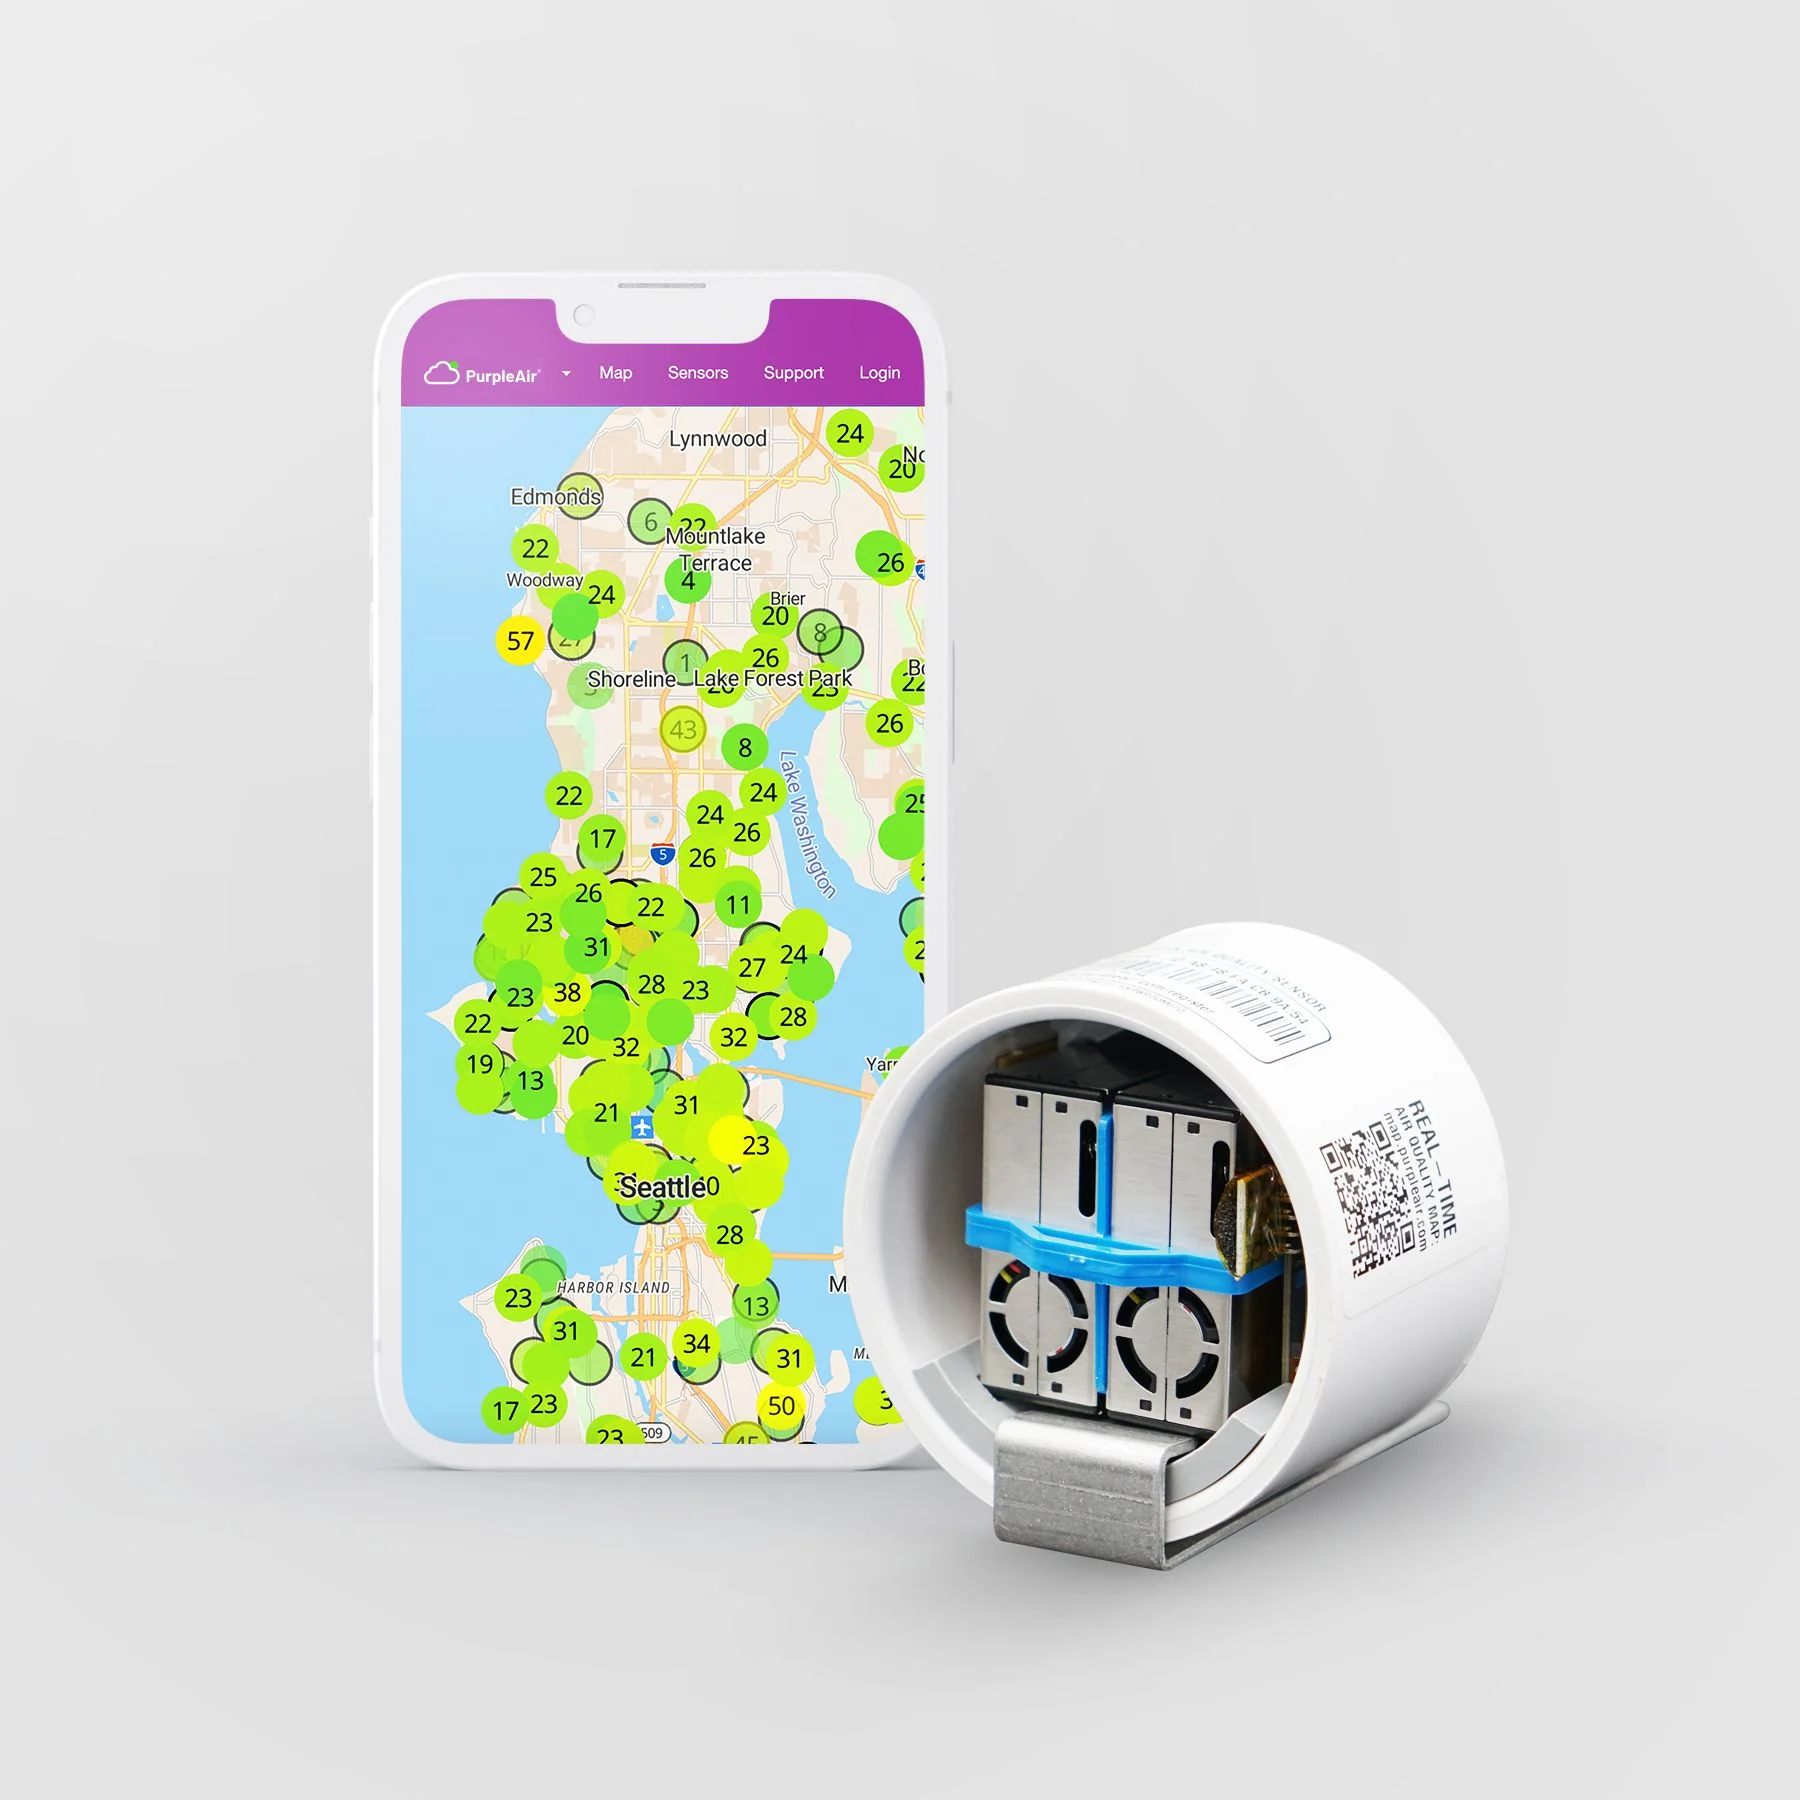
\includegraphics[width=0.62\linewidth]{purple}
\captionof{figure}{Low cost, portable PM2.5 monitor from PurpleAir. Image from PurpleAir}
\end{center}

\begin{center}
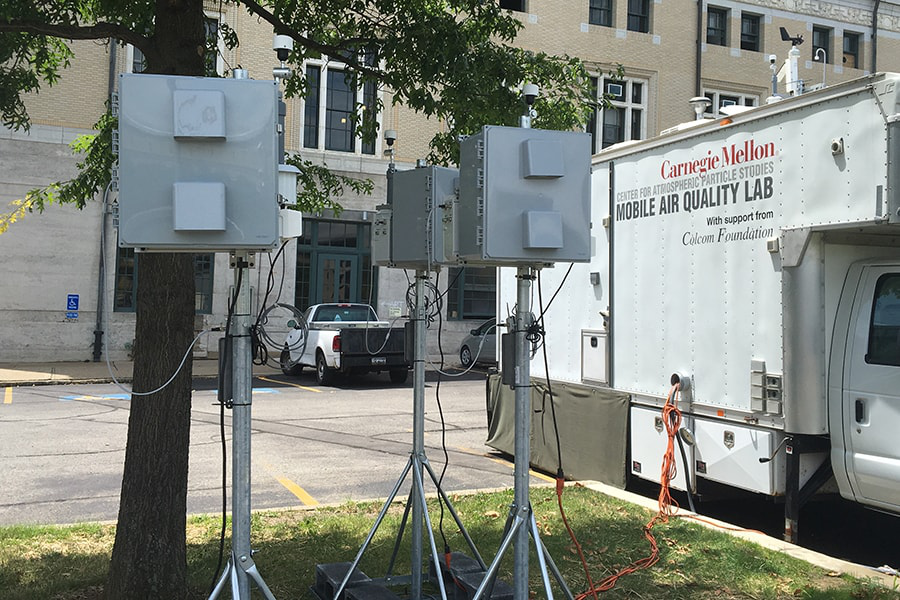
\includegraphics[width=0.62\linewidth]{ramp}
\captionof{figure}{Example of a Multipollutant, RAMP sensor. Image from Carnegie Mellon University}
\end{center}

}


%----------------------------------------------------------------------------------------

\end{poster}

\end{document}
